\documentclass[openany, letterpaper, 11pt]{book}

%%%% ----------------------------------------------------------------------
%%%% 0. PAQUETES ESENCIALES
%%%% ----------------------------------------------------------------------

%%% Paquete tikz
	\usepackage{tikz}

%%%     Librerías a emplear de tikz
		\usetikzlibrary{calc, shapes.geometric, arrows}

%%% Paquete pgfplots
	\usepackage{pgfplots}

%%%     Definición de las propiedades del tipo de pgfplot
		\pgfplotsset{compat=1.8}

%%% Paquete para colores en el documento
	\usepackage{xcolor}
	\usepackage{color}

%%%     Definición de colores a emplear en el documento 
		\definecolor{color1}{RGB}{45, 0, 31} % <-- Gama de rojo oscuro
		\definecolor{color2}{RGB}{147, 0, 31} % <-- Gradiente del color 1
		\definecolor{color3}{RGB}{139, 25, 0} % <-- Gradiente del color 2
		\definecolor{color4}{RGB}{247, 25, 0} % <-- Gradiente del color 3
		\definecolor{grisOscuro}{RGB}{100, 100, 100} % <-- Color gris
		\definecolor{grisClaro}{RGB}{180, 180, 190} % <-- Color gris claro


%%%% ----------------------------------------------------------------------
%%%% 1. PAQUETES DE CONFIGURACIÓN DE PÁGINA
%%%% ----------------------------------------------------------------------

%%% Definición de codificación
	\usepackage[utf8]{inputenc}

%%% Definición del tipo de fuente
	\usepackage[T1]{fontenc}

%%% Definición del lenguaje de escritura
	\usepackage[spanish]{babel}

%%%     Definición del tipo de separador decimal
		\spanishdecimal{.}

%%% Definición de la fuente principal de trabajo
	\usepackage{FiraSans}
	\usepackage{kerkis}

%%% Configuración de los márgenes de página
	\usepackage[margin=1in]{geometry}

%%% Configuración del espaciado de renglones en zonas específicas y global
	\usepackage{setspace} 
		\renewcommand{\baselinestretch}{1.15} % <--- Configuración global
%		\renewcommand{\parskip}{12}
		\setlength\parskip{12pt}

%%% Adición para cajas de colores y teoremas
	\usepackage{tcolorbox}


%%%% ----------------------------------------------------------------------
%%%% 2. PAQUETES MATEMÁTICOS
%%%% ----------------------------------------------------------------------

%%% Paquetes AMS 
	\usepackage{amssymb}
	\usepackage{amsfonts}
	\usepackage{cancel}
	\usepackage{amsmath}
	\usepackage{latexsym}


%%%% ----------------------------------------------------------------------
%%%% 3. PAQUETES PARA FLOTANTES
%%%% ----------------------------------------------------------------------

%%% Configuración de flotantes en cualquier situación  
	\usepackage{float}

%%% Ajuste de columnas y de tablas
	\usepackage{array}

%%%     Adición de nuevos estilos de columnas
		\newcolumntype{C}[1]{>{\centering\let\newline\\\arraybackslash\hspace{0pt}}m{#1}}

%%% Ajuste de títulos de flotantes
	\usepackage{caption}

%%%     Declaración de ajustes para los captions de los flotantes
		\DeclareCaptionFont{colorlabel}{\color{color1}}
		\captionsetup{labelfont={sf, bf, colorlabel}}

%%% Adición de gráficas en diferentes formatos
	\usepackage{graphicx}

%%% Para alinear varias figuras en un solo conjunto
	\usepackage{subfigure}

%%% Para la adición de tablas que sobrepasan una página del documento
	\usepackage{longtable}

%%% Unión de varias filas en una sola 
	\usepackage{multirow}

%%% Encabezado tipo libro en tablas
	\usepackage{booktabs}

%%% Adición de color a las tablas, tanto en líneas (hline), como también a las celdas y filas de una tabla
	\usepackage{colortbl}

%%% Ajuste del espaciado en tablas, y el color de las líneas de separación en tablas
	\renewcommand{\arraystretch}{1.4}
	\arrayrulecolor{color1}

%%% Adición de notas en las tablas
	\usepackage[flushleft]{threeparttable}


%%%% ----------------------------------------------------------------------
%%%% 4. AJUSTE DE BIBLIOGRAFÍA DEL DOCUMENTO
%%%% ----------------------------------------------------------------------

%%% Paquete NatBIB
\usepackage{natbib}

%%% Paquete cite
\usepackage{cite}


%%%% ----------------------------------------------------------------------
%%%% 5. REDEFINICIÓN DE NUEVOS COMANDOS PARA ESTILIZACIÓN
%%%% ----------------------------------------------------------------------

\usepackage{lipsum}





\begin{document}
	
	
%%% -----------------------------------------------------------------------
%%% Adición de portada, TOC, TOT, TOF
%%% -----------------------------------------------------------------------

	%%%% ------------------------------------------------------------------
%%%% PORTADA DEL MANUAL DE TRABAJO
%%%% ------------------------------------------------------------------

\begin{titlepage}
	\begin{tikzpicture}[remember picture, overlay, shift=(current page.south west)]
		\def\x{0.8}
		\begin{scope}[x={(current page.south east)}, y={(current page.north west)}]
			
			%%%% Fondo general del documento
			\node[] at (current page.center) {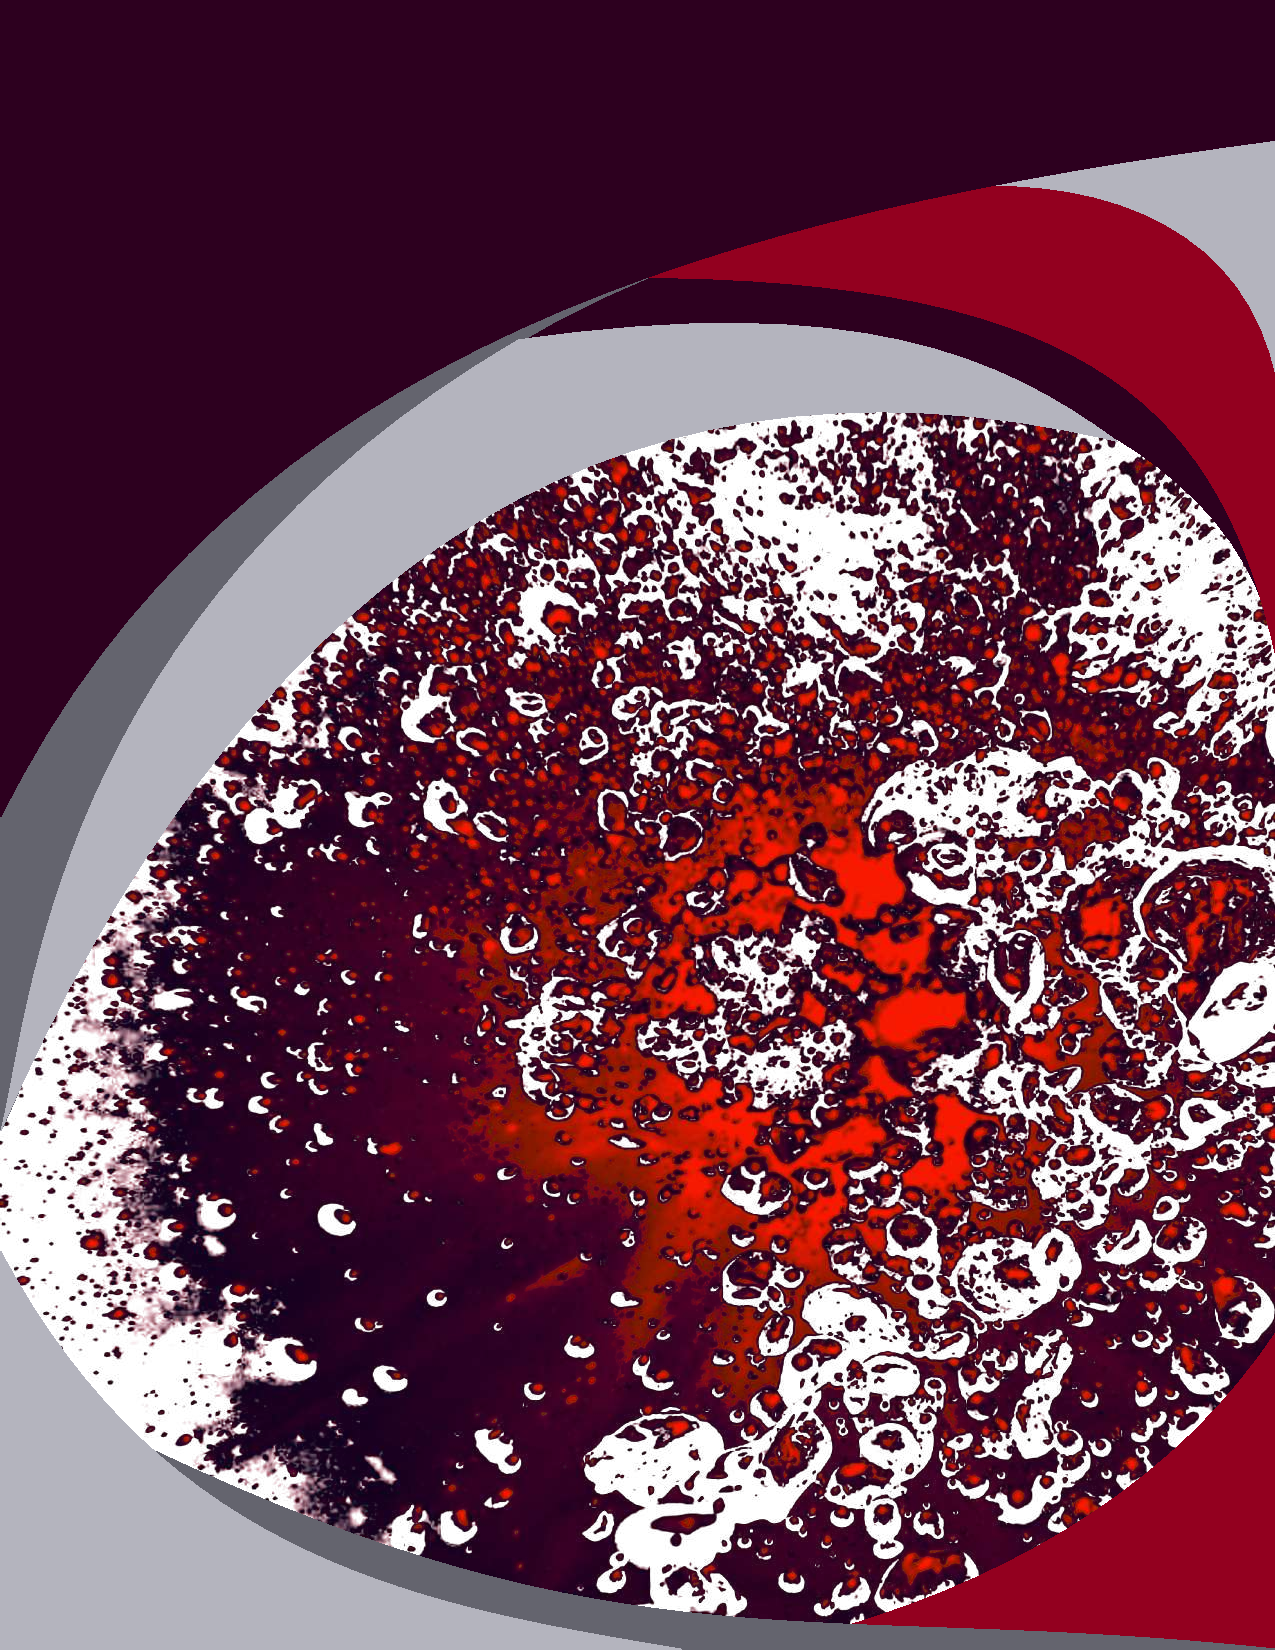
\includegraphics[scale=1.01]{Imagenes/bgManual}};
			
			%%%% Ubicación de los títulos del manual
			\node[font=\firabook\bfseries\fontsize{40}{41}\selectfont, text=white, anchor=north west, align=flush left, text width=14cm] (title) at (0.04, 0.985) {\MakeUppercase{Dinámica de Fluidos Computacional:}}; 
			
			%	\draw[white, line width=5pt] ([xshift=-3.75cm, yshift=-0.35cm]title.south east) -- ([xshift=-0.5cm, yshift=-0.35cm]title.south west);
			
			\node[font=\fontsize{25}{26}\selectfont\itshape, text=white, anchor=north west, text width=8cm, align=flush left] at ([yshift=-0.35cm]title.south west) {Teoría y manejo de OpenFOAM};
			
			%%%% Adición de logo de la UD en la parte inferior
			\node [anchor=south west] (logoUD) at (0.005, 0.005) {
\includegraphics[width=1.25cm]{Imagenes/logoUDRojo}};
			
			\node [anchor=west, font=\bfseries\footnotesize, align=flush left, inner sep=0pt, text=color1, scale=\x] (nameUp) at ([yshift=0.3cm]logoUD.east) {UNIVERSIDAD DISTRITAL};
			\node [anchor=north west, font=\bfseries\fontsize{7.75}{8}\selectfont, inner sep=0pt, align=flush left, text=color1, scale=\x] (nameBelow) at ([yshift=-1.5pt]nameUp.south west) {FRANCISCO JOSÉ DE CALDAS};
			
			\draw[color1, line width=0.5pt, scale=\x] ([yshift=-1.5pt]nameBelow.south west) -- ([yshift=-1.5pt, xshift=0.25cm]nameBelow.south east);
			
			\node [font=\bfseries\fontsize{6.5}{7}\selectfont, inner sep=0pt, align=flush left, text=color1, text width=4cm, anchor=north west, scale=\x] (facultad) at ([yshift=-5pt]nameBelow.south west) {Facultad del Medio Ambiente y Recursos Naturales};
			
		\end{scope}
	\end{tikzpicture}
\end{titlepage}
	
%	\tableofcontents % <-- Emplear cuando se tengan secciones realizadas
%	\listoftables % <-- Emplear para cuando se tengan tablas realizadas
%	\listoffigures % <-- Emplear para cuando se tengan figuras realizadas


		
	
\section{Introducción}

\lipsum[0-10]

\end{document}
